% ==============================================================================
% SLIDES - SEMANA 03: TEORIA GERAL DOS DISPOSITIVOS INDUSTRIAIS (SENSORES, ATUADORES E CLP/IHM)
% ==============================================================================

% 1. CAPA
\senaicover
  {Teoria Geral dos Dispositivos Industriais}
  {Sensores Avançados, RFID, Atuadores Pneumáticos/Elétricos, CLP e Ciclo de SCAN}
  {Unidade Curricular: Automação Industrial}
  {Prof. André Souza}

% 2. AGENDA DA AULA
\begin{senaiframe}{Visão Geral \& Agenda}{Estrutura do Conteúdo}
  \begin{columns}[t]
    \begin{column}{0.48\textwidth}
      \begin{tcolorbox}[senaibluecard, title={1. Sensoriamento Avançado}]
        \begin{itemize}
          \item Fotoelétricos (Barreira, Refletivo, Difuso).
          \item Ultrassônicos (\textit{Time-of-Flight}).
          \item Rastreabilidade RFID (ISO 15693).
        \end{itemize}
      \end{tcolorbox}
      \vspace{4pt}
      \begin{tcolorbox}[senaiambercard, title={3. Arquitetura do CLP}]
        \begin{itemize}
          \item Estrutura de Hardware e Optoacopladores.
          \item Entradas e Saídas Analógicas ($4-20\text{ mA}$).
        \end{itemize}
      \end{tcolorbox}
    \end{column}
    \begin{column}{0.48\textwidth}
      \begin{tcolorbox}[senairedcard, title={2. Atuadores Industriais}]
        \begin{itemize}
          \item Pneumática (Unidade FRL, Válvulas 5/2).
          \item Inversores de Frequência (VFD / PWM).
          \item Servomotores em Malha Fechada.
        \end{itemize}
      \end{tcolorbox}
      \vspace{4pt}
      \begin{tcolorbox}[senaigreencard, title={4. Ciclo de SCAN \& IHM}]
        \begin{itemize}
          \item O Ciclo de SCAN Determinístico (4 Fases).
          \item Memória de Imagem PII e PIO.
          \item Interfaces Homem-Máquina (IHM).
        \end{itemize}
      \end{tcolorbox}
    \end{column}
  \end{columns}
\end{senaiframe}

% 3. SENSORES FOTOELÉTRICOS
\begin{senaiframe}{Sensores Ópticos}{Sensores Fotoelétricos Industriais}
  Utilizam a emissão e recepção de feixes de luz modulada (infravermelha ou laser) para detectar alvos a longas distâncias.

  \vspace{4pt}
  \begin{itemize}
    \item \textbf{Modulação de Luz:} O emissor oscila o feixe óptico em alta frequência para evitar que a iluminação ambiente do galpão fabril cause disparos falsos no receptor.
    \item \textbf{Vantagens:} Longo alcance de detecção e alta velocidade de resposta eletrônica.
  \end{itemize}
\end{senaiframe}

% 4. INFOGRÁFICO SENSORES FOTOELÉTRICOS
\begin{senaiframe}{Tipos de Ópticos}{Infográfico Comparativo de Fotoelétricos}
  \begin{columns}[c]
    \begin{column}{0.55\textwidth}
      \centering
      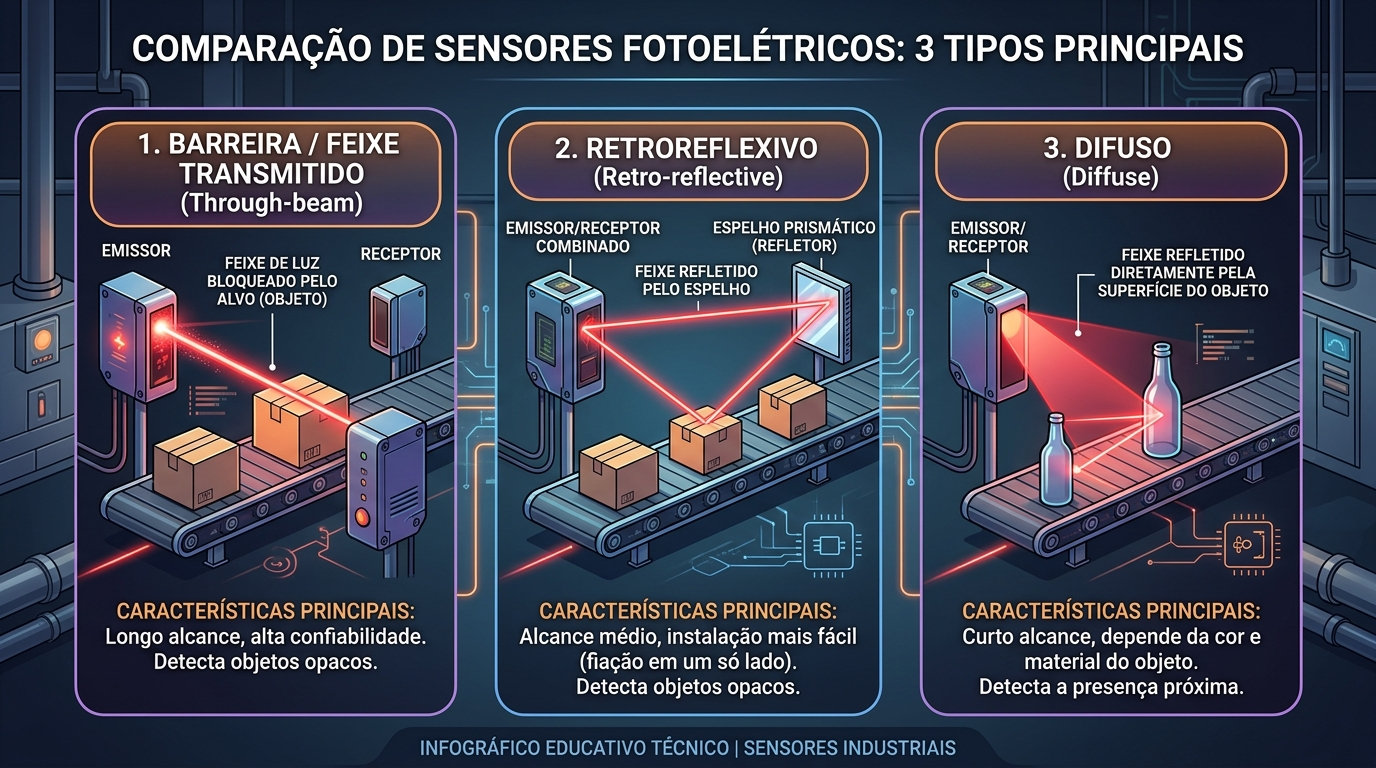
\includegraphics[width=\textwidth, height=0.72\textheight, keepaspectratio]{../aulas/img/sensores_fotoeletricos.jpg}
    \end{column}
    \begin{column}{0.42\textwidth}
      \small
      \textbf{Principais Modelos:}
      \begin{itemize}
        \item \textbf{Barreira (Through-beam):} Emissor e receptor separados. Maior alcance ($\sim 50\text{m}$).
        \item \textbf{Retroreflexivo:} Utiliza espelho prismático. Cabeamento em um só lado.
        \item \textbf{Difuso:} Reflete diretamente na superfície do objeto.
      \end{itemize}
    \end{column}
  \end{columns}
\end{senaiframe}

% 5. TECNOLOGIAS ÓPTICAS AVANÇADAS
\begin{senaiframe}{Recursos Ópticos}{Filtro Polarizado e Supressão de Fundo}
  \begin{block}{\textbf{Filtro Polarizado (Retroreflexivo)}}
    Utiliza filtros de polarização cruzada. A luz do espelho prismático gira $90^\circ$, permitindo ao receptor diferenciar a reflexão do espelho de um objeto metálico brilhante (evitando falsos disparos).
  \end{block}

  \vspace{4pt}
  \begin{block}{\textbf{Supressão de Fundo (Background Suppression)}}
    Sensores difusos avançados medem o ângulo da luz refletida através de receptores PSD. Permitem detectar uma peça escura próxima e ignorar um fundo brilhante distante.
  \end{block}
\end{senaiframe}

% 6. SENSORES ULTRASSÔNICOS
\begin{senaiframe}{Sensoriamento Acústico}{Sensores Ultrassônicos e Time-of-Flight (ToF)}
  Detectam alvos sólidos ou líquidos emitindo pulsos de ondas de som de alta frequência ($200\text{ kHz}$ a $400\text{ kHz}$) e medindo o tempo de eco:

  $$d = \frac{v_{\text{som}} \cdot t_{\text{eco}}}{2}$$

  \begin{itemize}
    \item \textbf{Independência Óptica:} Detectam materiais totalmente transparentes (garrafas de vidro, água, filmes plásticos).
    \item \textbf{Compensação Térmica Integrada:} Possuem termistor NTC embutido para corrigir variações da velocidade do som com a temperatura ambiente.
    \item \textbf{Zona Cega (Blind Zone):} Região física nos primeiros centímetros à frente da face sensora onde medições são impossíveis.
  \end{itemize}
\end{senaiframe}

% 7. RASTREABILIDADE POR RFID
\begin{senaiframe}{Identificação Automática}{Identificação por Rádio Frequência (RFID)}
  Permite a leitura e escrita sem contato de dados de produção diretamente em microchips acoplados aos produtos na linha \textbf{Smart N1}.

  \vspace{4pt}
  \begin{itemize}
    \item \textbf{Tags Passivas:} Energizadas por indução eletromagnética da antena do leitor.
    \item \textbf{Estrutura de Memória:}
      \begin{itemize}
        \item \textbf{UID (Unique Identifier):} Código único hexadecimal de fábrica (ROM).
        \item \textbf{User Memory:} Bloco regravável onde o CLP salva a receita do produto e o histórico de testes de qualidade.
      \end{itemize}
    \item \textbf{Padrões:} HF ($13,56\text{ MHz}$ - ISO 15693) e UHF ($900\text{ MHz}$ - EPC Gen2).
  \end{itemize}
\end{senaiframe}

% 8. ATUADORES PNEUMÁTICOS
\begin{senaiframe}{Sistemas de Potência}{Atuadores Pneumáticos e Válvulas Solenoide}
  Transformam a energia do ar comprimido ($6\text{ bar}$) em trabalho mecânico linear.

  \vspace{4pt}
  \begin{itemize}
    \item \textbf{Unidade FRL:} Filtro de umidade, Regulador de Pressão e Lubrificador.
    \item \textbf{Cilindro de Dupla Ação:} Avanço e retorno comandados pneumaticamente pelas duas câmaras.
    \item \textbf{Válvula Solenoide 5/2 Vias:} Válvula direcional de 5 conexões e 2 posições, acionada por solenoides elétricas de $24\text{V DC}$ conectadas ao CLP.
  \end{itemize}
\end{senaiframe}

% 9. ACIONAMENTOS ELÉTRICOS DE POTÊNCIA
\begin{senaiframe}{Acionamentos Elétricos}{Motores Trifásicos, Inversores VFD e Servos}
  \small
  \begin{itemize}
    \item \textbf{Motor Assíncrono Trifásico (MIT):} Cavalo de batalha da indústria. Velocidade síncrona $N_s = \frac{120 \cdot f}{P}$.
    \item \textbf{Inversor de Frequência (VFD):}
      \begin{itemize}
        \item Estágios: Retificador AC/DC $\rightarrow$ Barramento DC $\rightarrow$ Inversor IGBT PWM.
        \item Permite controle suave de velocidade e rampas de aceleração, eliminando picos de partida.
      \end{itemize}
    \item \textbf{Servomotores \& Servo Drivers:}
      \begin{itemize}
        \item Operam em \textbf{malha fechada} com encoder de alta resolução no eixo, permitindo controle milimétrico de posição e torque.
      \end{itemize}
  \end{itemize}
\end{senaiframe}

% 10. CONTROLADORES INDUSTRIAIS (CLP)
\begin{senaiframe}{Arquitetura de Hardware}{Controladores Lógicos Programáveis (CLP)}
  Computador industrial determinístico projetado para operação contínua 24/7.

  \vspace{4pt}
  \begin{itemize}
    \item \textbf{CPU:} Processador e sistema operacional de tempo real (RTOS).
    \item \textbf{Isolamento Óptico (Optoacopladores):} Protege a eletrônica interna da CPU contra surtos de tensão e ruídos elétricos vindos dos sensores de campo.
    \item \textbf{Módulos de E/S Analógicas:} Interface com transmissores padronizados de $4\text{ a }20\text{ mA}$ ou $0\text{ a }10\text{ V}$.
  \end{itemize}
\end{senaiframe}

% 11. INFOGRÁFICO CICLO DE SCAN DO CLP
\begin{senaiframe}{Determinismo Temporal}{O Ciclo de SCAN do CLP}
  \begin{columns}[c]
    \begin{column}{0.55\textwidth}
      \centering
      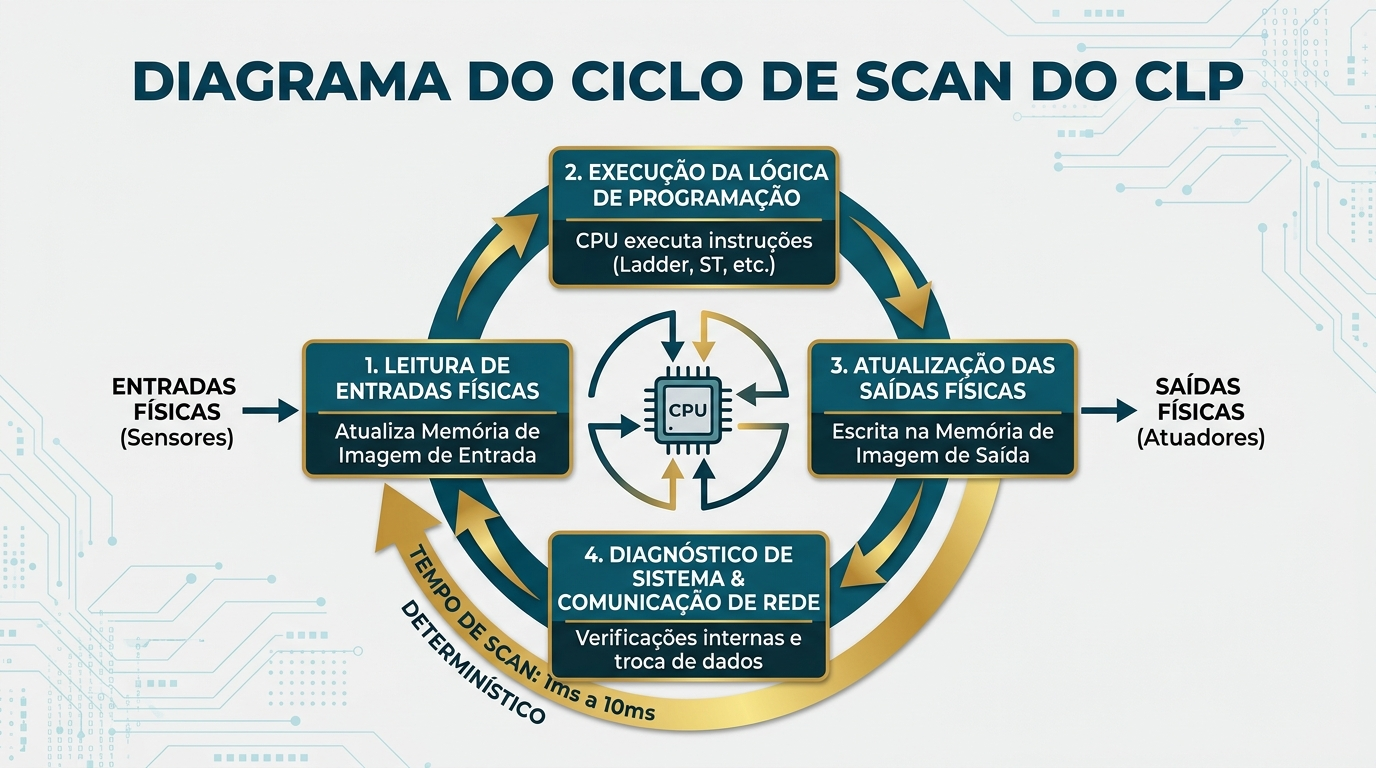
\includegraphics[width=\textwidth, height=0.72\textheight, keepaspectratio]{../aulas/img/ciclo_de_scan_clp.jpg}
    \end{column}
    \begin{column}{0.42\textwidth}
      \small
      \textbf{As 4 Etapas do SCAN:}
      \begin{enumerate}
        \item \textbf{Leitura das Entradas:} Copia o campo para a Memória PII.
        \item \textbf{Execução da Lógica:} Roda o programa ST/Ladder.
        \item \textbf{Atualização das Saídas:} Escreve a Memória PIO no campo.
        \item \textbf{Comunicação \& Diagnóstico.}
      \end{enumerate}
    \end{column}
  \end{columns}
\end{senaiframe}

% 12. IHMs E FIXAÇÃO TEÓRICA
\begin{senaiframe}{Interface e Revisão}{Interfaces Homem-Máquina (IHM) \& Fixação}
  \begin{block}{\textbf{Interface Homem-Máquina (IHM / HMI)}}
    Telas industriais para visualização de sinóticos animados, alteração de parâmetros de receita e histórico de alarmes em tempo real.
  \end{block}

  \vspace{4pt}
  \small
  \textbf{Questão de Fixação:} Por que a leitura das entradas no CLP é copiada para uma "Memória de Imagem" no início do ciclo em vez de ser lida diretamente a cada instrução do código?  
  \textit{Resposta:} Para garantir \textbf{determinismo e consistência de dados} durante toda a varredura do programa.
\end{senaiframe}
